% !TEX root = DataDrivenBayes.tex

\section*{Case study 3: A descriptive approach can be relevant even when questions about optimality are not} 

The first two case studies differed in several respects and led us to different theoretical conclusions about the optimality of human reasoning in the two problems considered, but one attribute they share is the very fact that optimal models and descriptive models are both applicable to the problem. This is not always the case. In many situations a Bayesian model serves a useful purpose even when no clear notion of ``optimality'' seems to apply. Probabilistic topic models \cite{steyvers_probabilistic_2007}, for instance, are often used as tools for exploring human semantic knowledge, but the scientific utility of these models is not generally taken to justify any claim about human {\it optimality}. In such situations it may be convenient to use a Bayesian model, but the primary intention is to use the model as a tool. Applying a Bayesian model in this fashion aligns naturally with the descriptive Bayesian framework, because the researcher merely claims that the Bayesian model produces similar behavior to humans and does not use a good model fit to justify an optimality claim. 

Our third case study presents one such example, using an existing Bayesian model of inductive generalization as a tool to explore the hypotheses that might guide people's intuitions in simple reasoning problems. The goal here is to highlight the fact that very often researchers can use descriptive Bayesian models productively, even in situations where questions about the ``optimality'' of human cognition do not seem especially relevant to the research question. 






\subsection{Inductive generalization as Bayesian reasoning}

The Bayesian theory of generalization developed by \citeA{Tenenbaum2001} (henceforth TG1) formalized the problem of inductive generalization in the following way. Suppose a learner is told that some set of entities $X = \lbrace x_1,. . ., x_n \rbrace$ all possess some property $P$, and is asked to infer whether a new entity $y$ also shares that property. Suppose also that the learner is equipped with some {\it hypothesis space} $\mathcal{H}$ that consists of all hypotheses $h$ that the learner considers for the extension of the property $P$, and a prior $P(h)$ over these hypotheses that describes how plausible the learner considers each hypothesis to be before any data are observed. When told that the entities $X$ possess property $P$, the learner updates their beliefs via Bayes' rule:
$$ 
P(h | X) \propto P(h) \prod_{i} P(x_i | h)
$$
where $P(x_i | h)$ describes the probability that the entity $x_i$ would be observed to have property $P$ if hypothesis $h$ describes the true extension of that property. Given this posterior distribution the probability that the property extends to the novel entity $y$ is computed by summing the posterior probabilities of all hypotheses $h$ that assert that $y$ possesses $P$:
\begin{equation}
\label{eq:generalization}
P(y \mid X) = \sum_{h:y \in h} P(h \mid X).
\end{equation}
The central feature of the Bayesian generalization model developed by TG1 is the choice of likelihood function, which they referred to as {\it strong sampling}, and assumes that the observed entities are sampled {\it from} the set of entities that possess property $P$. In particular, if observations are sampled randomly from this set, then the probability of observing any specific item $x$ given that the true extension of $P$ is described by hypothesis $h$ is given by
\begin{equation}
P(x \mid h) = \begin{cases}
 \dfrac{1}{\vbars{h}} & \text{if $x\in h$},\\
 0& \text{otherwise}.
\end{cases}
\end{equation}
where $\vbars{h}$ is the {\it size} of the hypothesis $h$, and for hypotheses $h$ that consist of only a finite number of entities the size of the hypothesis corresponds to the number of entities that it contains. 
 
When introducing the model, TG1 noted that this strong sampling model is the central feature of the theory. There are other Bayesian induction models that rely on different sampling models \cite{heit_bayesian_1998,VoorspoelsINPRESS,navarro2012} and there are empirical results suggesting that people can change their sampling assumptions to suit the context \cite{RansomINPRESS,VoorspoelsINPRESS,gweon_infants_2010}. Nevertheless, there is considerable evidence that it works well as a default model for inductive generalization \cite{sanjana_bayesian_2003}. 

\subsection{The hypothesis space problem}

The biggest practical difficulty that arises when applying the Bayesian generalization model is the fact that---although it provides an unambiguous specification of the likelihood function $P(x|h)$---it places few if any constraints on the choice of hypothesis space $\mathcal{H}$ or the prior distribution $P(h)$ defined over that space. The original work by \citeA{shepard_toward_1987} assumed that hypotheses corresponded to connected regions within a suitably formulated psychological space \cite<and estimated by multidimensional scaling or similar methods:>{torgerson_theory_1958,borg_modern_2005}. However, TG1 proposed that the Bayesian generalization model could be applied more widely than this, including in cases where the stimuli are defined in terms of a set of discrete features \cite<estimated using additive clustering or similar methods: >{shepard_additive_1979,lee_generating_2002,navarro2008}.

This extension of the model is one of the more innovative elements to the TG1 work, but introduces a problem for the researcher. If the goal is to study how people generalize from stimuli, what hypothesis space should we assume they use to guide their inferences and what priors over those hypotheses are sensible? The original TG1 paper notes this issue, but does not propose a solution. In applications of the model researchers have tended to fall back on the traditional solution of trying to infer mental representations (and by extension hypothesis spaces) from a set of similarity judgments. For instance, \citeA{sanjana_bayesian_2003} used a hierarchical clustering method to infer a taxonomic tree for a set of animals, whereas \citeA{RansomINPRESS} used a variation of additive clustering to infer a set of hypotheses that allowed for cross-cutting categories. In both cases, the authors relied heavily on the assumption that a set of similarity judgments produced by different participants in a different experiment can be relied upon to constrain the Bayesian generalization model.

An alternative approach to the problem is to estimate a hypothesis space $\mathcal{H}$ from the generalization judgments themselves. Multidimensional scaling and additive clustering are statistical techniques that rely upon psychological theories of similarity judgment (e.g., geometric similarity models, feature contrast models) to provide the link between empirical data and the inferred mental representation. However, if the goal is to learn something about the hypotheses that constrain people's generalizations, it seems to make more sense to use a psychological theory of generalization to do to the work. 


\subsection*{Experiment}

The data for this case study come from a property induction task \cite<e.g.,>{osherson_category-based_1990}. In it, participants are presented with one or more examples that share a novel property and are then asked to rate the probability that additional exemplars also possess that property. Data were collected from 762 workers on Amazon Mechanical Turk who were paid \$0.50 for completing the $10$-minute study. After a pretest designed to ensure that people understood the task, they were given the following question: 

\begin{quote}
{\it In the past, scientists discovered that all $\mathbf{A}$ have an enzyme called Enzyme-Q. What is the probability that each of the following animals also have Enzyme-Q?}
\end{quote}

\noindent
The known exemplar $\mathbf{A}$ was one of the following 20 mammals: \stimulus{bats, beavers, chimps, cows, dolphins, elephants, gorillas, horses, kangaroos, koalas, mice, pandas, polar bears, rabbits, rhinos, seals, squirrels, tigers, whales}, or \stimulus{wolves}. People were asked to give probability judgments for all 20 the mammals by moving a slider between 0\% and 100\%. After providing probability judgments for all of the mammals, all of the sliders were reset to 0\% and people were given the following additional information: 
\begin{quote}
{\it Later, scientists discovered that in addition to $\mathbf{A}$, all $\mathbf{B}$ also have Enzyme-Q. Given this new information, what is the probability that each animal has Enzyme-Q?}
\end{quote}

\noindent
The first exemplar \textbf{A} remained unchanged, and the second exemplar \textbf{B} was one of the remaining mammals other than \textbf{A}. Trials were balanced so that each of the 190 possible combinations of two mammals occurred approximately four times across all participants.


\subsection*{Results}

We excluded from analysis 175 participants who either failed to follow the instructions on the pretest, or did not rate mammals as having a property with 100\% certainty when they were told the mammal had that property in the instructions. Results are based on analysis of the remaining 587 participants. 

\begin{figure}[p]
\begin{center}
\begin{tabular}{cc}
	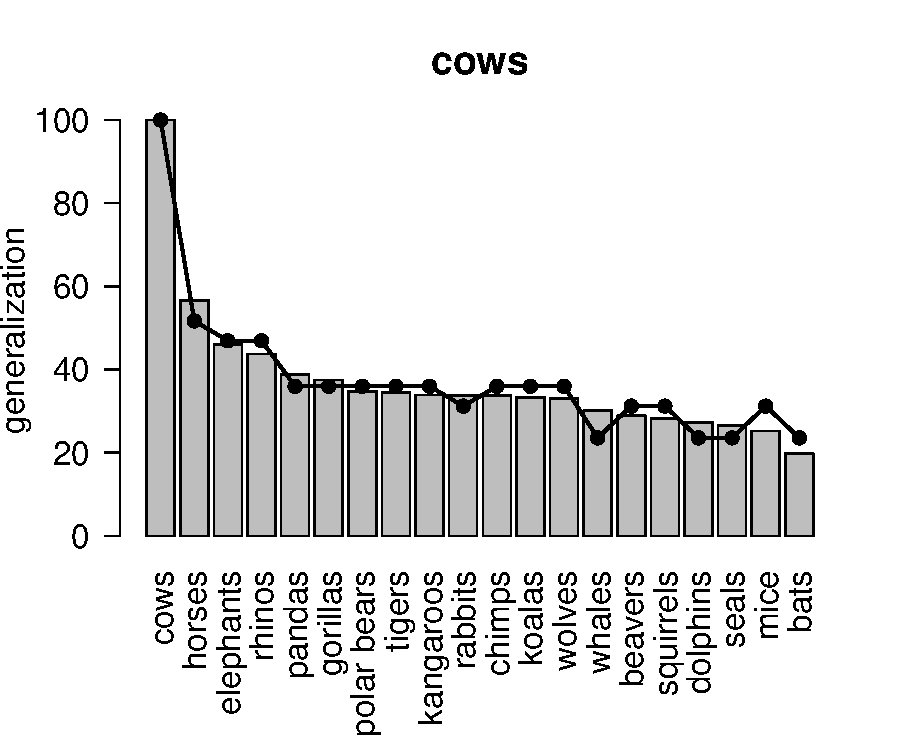
\includegraphics[width=6.5cm]{generalization_figs/cows.pdf} &
	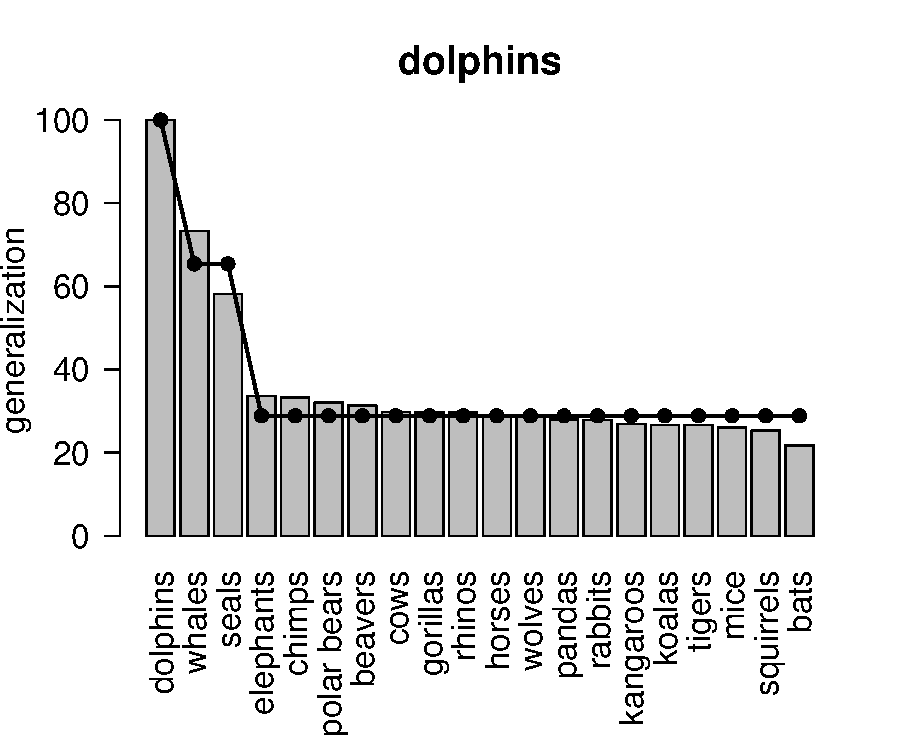
\includegraphics[width=6.5cm]{generalization_figs/dolphins.pdf} \\
	(a) & (d) \\
	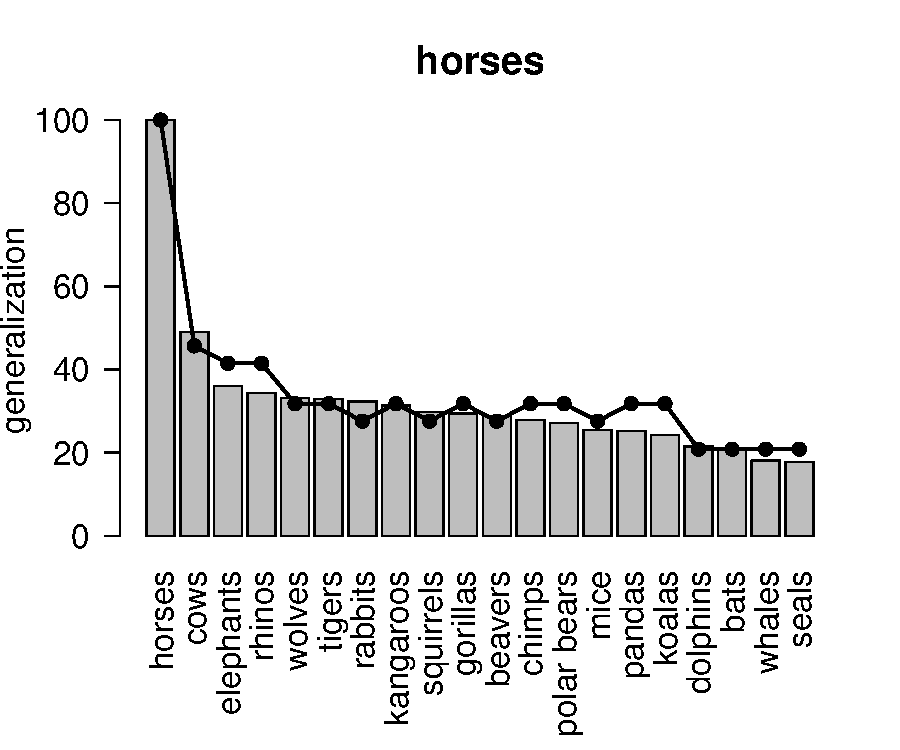
\includegraphics[width=6.5cm]{generalization_figs/horses.pdf} &
	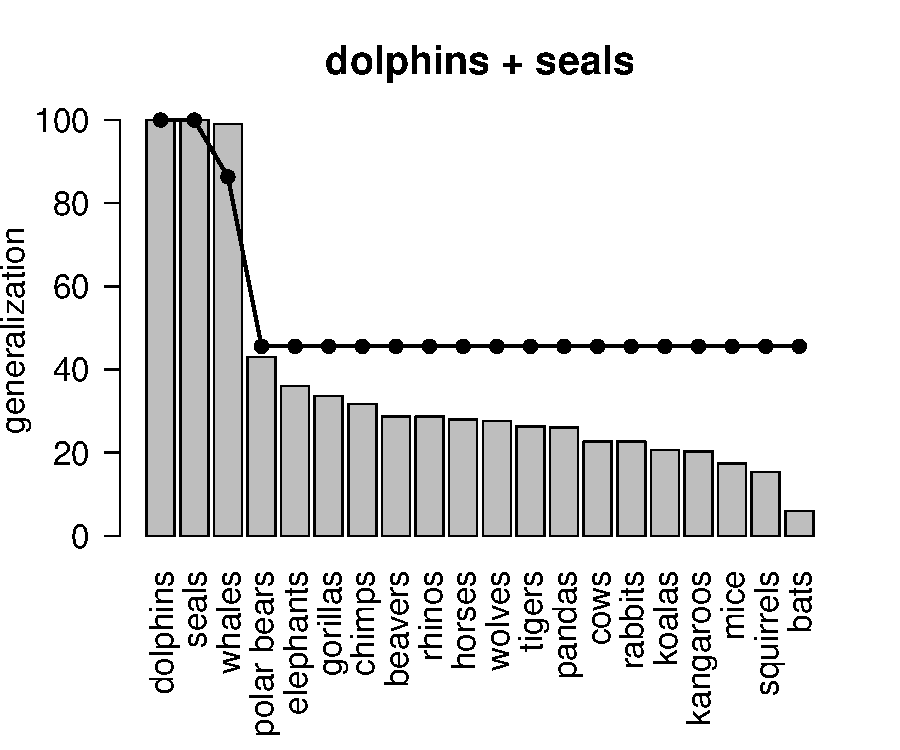
\includegraphics[width=6.5cm]{generalization_figs/dolphinsseals.pdf} \\
	(b) & (e) \\
	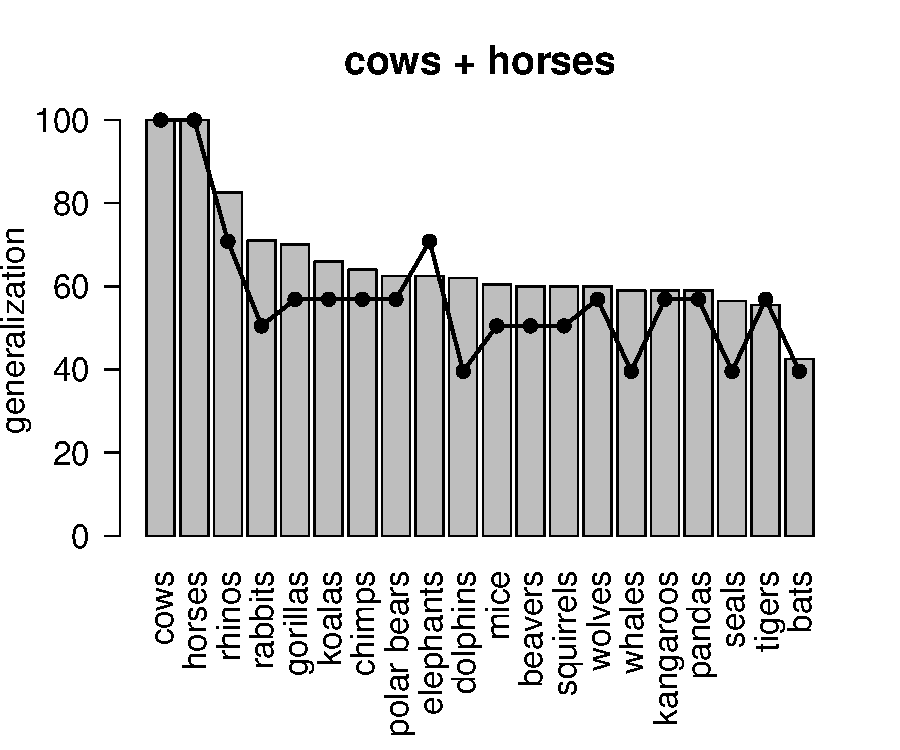
\includegraphics[width=6.5cm]{generalization_figs/cowshorses.pdf} &
	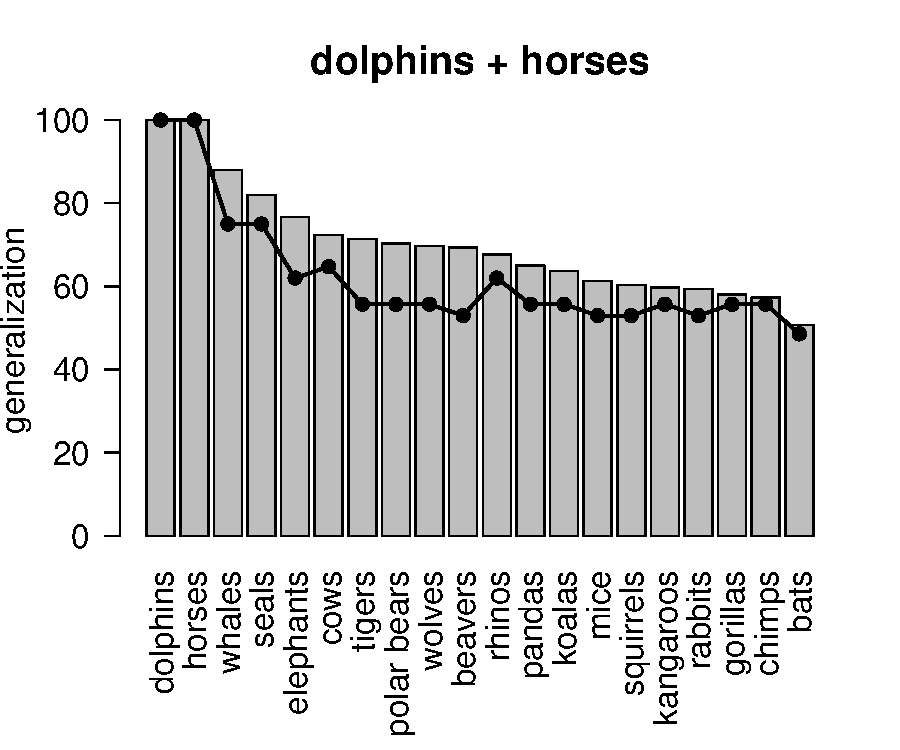
\includegraphics[width=6.5cm]{generalization_figs/dolphinshorses.pdf} \\	
	(c) & (f) \\
\end{tabular}
\vspace*{12pt}
\caption{Example generalization gradients produced by human participants (bars) compared to those estimated with the help of the Bayesian generalization model (solid lines). In each case, the title of the plot indicates which item(s) were known to possess Enzyme-Q, and the generalization targets are arranged in order of decreasing (human) generalization probability.}
\label{fig:gen_posterior_pred}
\end{center}
\end{figure}

	

%\begin{figure}[t]
%
%	\begin{subfigure}{1.0\textwidth}
%		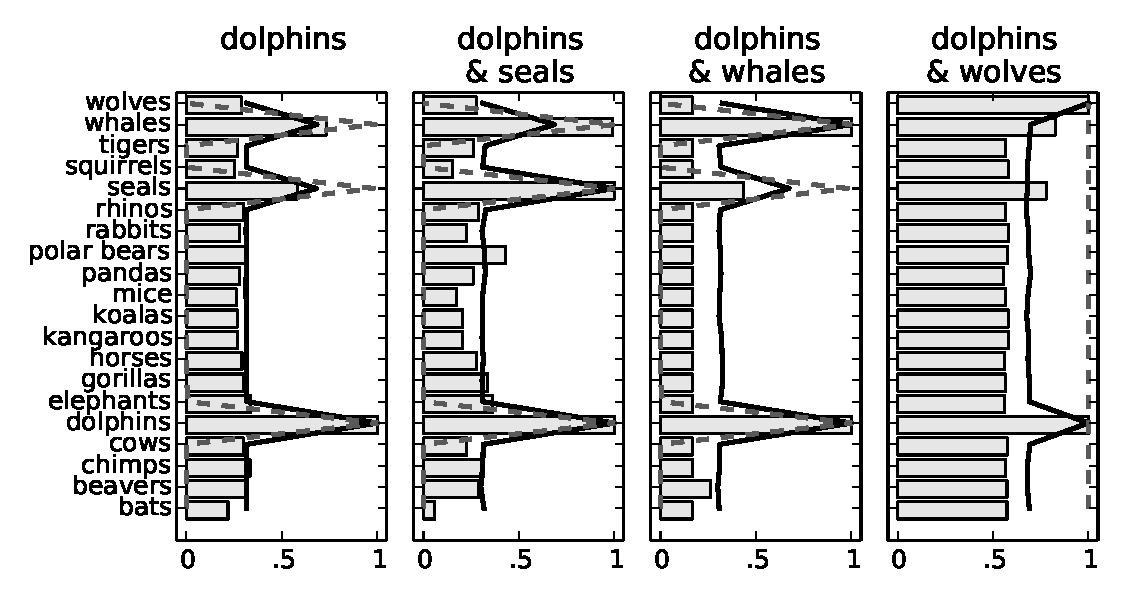
\includegraphics[width=.85\textwidth]{generalization_figs/comparison_dolphins.pdf}
%	\end{subfigure}
%	
%	\begin{subfigure}{1.0\textwidth}
%		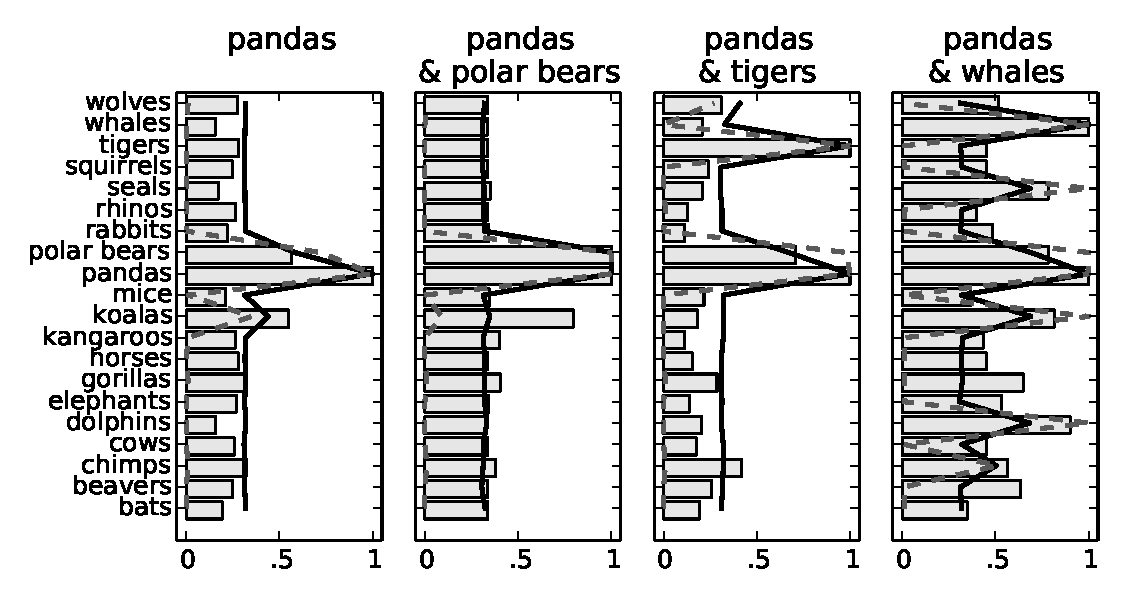
\includegraphics[width=.85\textwidth]{generalization_figs/comparison_pandas.pdf}
%	\end{subfigure}
%		
%	\caption{Mean human generalizations (bars) and posterior predictive responses with response noise (solid line) and without response noise (dashed line). }
%	\label{fig:gen_posterior_pred}
%\end{figure}


\bigskip
\subsubsection*{Human generalization data}

Representative generalization patterns from human participants are shown in Figure~\ref{fig:gen_posterior_pred}, and seem very sensible. When told that {\it cows} have Enzyme-Q people are most willing to extend that property to \stimulus{horses} (panel a) and vice versa (panel b). When told that Enzyme-Q is possessed by both \stimulus{cows} and \stimulus{horses}, people tended to extend the property far more widely (panel c): In this instance, our participants showed the {\it premise monotonicity} effect in which adding more positive examples causes people to generalize more widely. However, in other instances people showed the opposite {\it premise non-monotonicity} effect. For instance, compare the generalization gradients from \stimulus{dolphins} (panel d) to those from both \stimulus{dolphins} and \stimulus{seals} (panel e). The addition of the second exemplar increases the probability of some items (e.g., \stimulus{whales} shows premise monotonicity in this case) but decreases the probability of others (e.g., \stimulus{bats} shows non-monotonicity). 

This pattern, in which some generalizations show monotonicity effects and others non-monotonicity is generally explained by noting that some pairs of premise items tend to ``call attention'' to a specific category. Adding \stimulus{seals} to \stimulus{dolphins} strongly suggests that the true extension of the property is {\it marine mammals} and so the probability that \stimulus{whales} possess the property increases, and the probability hat \stimulus{bats} do so decreases. Moreover, when ``given'' the right set of categories upon which to base its inductive inferences, Bayesian generalization models capture this pattern perfectly well \cite<e.g.,>{RansomINPRESS}. However, this raises the question: How do we know {\it which} categories people people perceive to be relevant to the inductive generalization problem? It seems obvious that when reasoning about \stimulus{dolphins} and \stimulus{whales}, the category of {\it marine mammals} is relevant. This would explain the pattern of generalizations in panels (d)-(f) of Figure~\ref{fig:gen_posterior_pred}. Yet one might also have made the case that {\it farm animals} or {\it ungulants} might be perceived as especially relevant when reasoning about \stimulus{cows} or \stimulus{horses}, but when we compare panel (c) to panels (a) and (b) there is very little evidence for any non-monotonic inferences. 

\bigskip
\subsubsection*{Inferring a hypothesis space}

Given the above, how does the researcher work out which categories contributed to the learner's hypothesis space? This seems to be a natural context to apply probabilistic models: The Bayesian generalization model from TG1 supplies a theory that says, given {\it this} hypothesis space $\mathcal{H}$ and {\it that} prior $P(h)$ defined over it, then people should be expected to make {\it these} generalizations. We can use statistical methods to invert this: If we assume people produced those generalizations using this psychological model, what hypothesis space is required to support it? However, although the Bayesian framework is ideally suited to exactly this kind of work \cite<e.g.,>{navarro2008,kemp_discovery_2008}, it is not at all clear how any notion of {\it optimality} is relevant to this sort of problem. If we use the generalization model to infer a hypothesis space $\mathcal{H}$, does that mean that it is ``rational'' to use $\mathcal{H}$? Are we committed to a claim that people were reasoning rationally given those hypotheses? We are not at all convinced that either of these are true. Nevertheless, the underlying {\it descriptive} goal is an intriguing one: Can we use the TG1 model as a {\it tool} to learn something about the mental representations and hypotheses that people use to guide their generalizations? Bayesian optimality is quite irrelevant to this goal, but Bayesian description is very relevant indeed.  

Our approach is loosely based on the additive clustering model for extracting discrete categories from similarity judgments \cite{shepard_additive_1979} and adapted to the inductive generalization context using the model from TG1. We assume that the ``base'' hypothesis space $\mathcal{H}$ consists of a set of categories that can be described by the binary matrix $\mathbf{C}$ such that $c_{ik}=1$ if the $i$-th item belongs to the $k$-th category, and $c_{ik}=0$ if it does not. Some of the categories are fixed {\it a priori}: We assume that there exists a ``singleton'' category for each animal (e.g., one possibility is that the property holds for \stimulus{dolphins} only), and we assume that there exists a ``universal'' category (i.e., the property is true for all mammals). We impose no other {\it a priori} constraints on the structure of the category matrix $\mathbf{C}$. 

In order to construct the generalization probabilities for the Bayesian model, we follow \citeA{navarro2012} in allowing the model to {\it learn} the extent to which people use strong sampling or weak sampling, indexed using a single parameter $\theta$ (where $\theta=0$ implies weak sampling, and $\theta = 1$ implies strong sampling). Similarly, we follow \citeA{sanjana_bayesian_2003} in allowing {\it composite} hypothesis spaces in which the property in question might be possessed by two of the categories in $\mathbf{C}$.\footnote{There is nothing special about the number two. There is no reason why the hypothesis space could not include a hypothesis that property $P$ is characteristic of three or more categories. However, given that we never presented people with more than two premise items, the limitation to two seems sensible.} The model includes a free parameter $\gamma$ corresponding to the relative weight given to simple hypotheses where the property is assumed to be a characteristic of a single category, versus composite ones in which it is assumed to be a property of multiple categories. When $\gamma = 0$ all generalizations from multiple items rely on simple hypotheses only, whereas setting $\gamma = 1$ produces generalizations from composite hypotheses. The model is described in detail in Appendix C, along with details of how we estimate the category assignment matrix $\mathbf{C}$, the prior weights assigned to the categories, and the free parameters $\theta$ and $\gamma$.



\bigskip
\subsubsection*{Applying the model}

%wolves & 0.121 
%tigers & 0.089
%bats & 0.043
%rabbits & 0.0415
%rhinos & 0.0413 
%
%0.0391 :   pandas 
%0.0361 :   horses 
%0.0339 :   elephants 
%0.0336 :   koalas 
%0.0327 :   kangaroos 
%
%0.0308 :   squirrels 
%0.0293 :   mice 
%0.0284 :   cows 
%0.0264 :   polar bears 
%0.024 :   seals 
%
%0.0235 :   beavers 
%0.0166 :   dolphins 
%0.0146 :   whales 
%0.0113 :   chimps 
%0.0062 :   gorillas 



\begin{table}[t]
\caption{The categories inferred using the Bayesian generalization model. Additionally, the model included singleton categories (e.g., ``just dolphins'') and the universal category (i.e., ``all mammals''). \vspace*{6pt}}
\begin{center}
\begin{tabular}{p{7cm} | l | p{3cm}}
\textbf{hypothesis}	&	\textbf{prior} &	\textbf{interpretation}	\\
\hline
tigers, wolves & 0.089 & big predators \vspace*{3pt}\\
%bats, beavers, chimps, cows, dolphins, elephants, gorillas, horses, kangaroos, koalas, mice, pandas, polar bears, rabbits, rhinos, seals, squirrels, tigers, whales, wolves \vspace*{3pt}& 0.039 & all mammals \\
chimps, gorillas & 0.036 & primates \\
dolphins, seals, whales & 0.032 & marine mammals \\
bats, beavers, mice, rabbits, squirrels & 0.022 & rodents \\
koalas, pandas, polar bears & 0.022 & ``bears'' \\
cows, elephants, horses, rhinos & 0.019 & hoofed animals \vspace*{3pt}\\ 
beavers, chimps, cows, elephants, gorillas, horses, kangaroos, koalas, mice, pandas, polar bears, rabbits, rhinos, squirrels, tigers, wolves\vspace*{3pt} & 0.012 & non-marine, non-flying mammals  \\
chimps, cows, gorillas, horses, kangaroos, koalas, pandas, polar bears, tigers, wolves & 0.007 & medium-sized land mammals \\
\hline
\end{tabular}
\end{center}
\label{table:hypothesis_space}
\end{table}


The hypothesis space and priors that we estimated consists of the 9 categories listed in Table~\ref{table:hypothesis_space} and visualized in Figure~\ref{fig:hypothesis_space} (singleton categories and the universal category are omitted). The categories are generally sensible ones, and the generalization gradients that they produce are a reasonable approximation to human generalizations (e.g., solid lines in Figure~\ref{fig:gen_posterior_pred}). Some of the categories have a taxonomic basis (e.g., {\it primates}), others are superficial resemblances (e.g., \stimulus{koala} are unrelated to \stimulus{pandas}), and others are based on ecological roles (e.g., {\it large predator}). As a consequence, the overall structure of the categories people used to guide inductive inferences is non-hierarchical and cross-cutting. 

The parameter estimates are also revealing. The best fitting model parameters were $\theta=0.09$, which suggests that people tended not to rely on a strong sampling assumption. This pattern is consistent with earlier results \cite{navarro2012,RansomINPRESS}, and indeed has some resemblances with the ``conservative'' inferences in our first case study. The best fitting parameter value of $\gamma=0.91$ indicates that people had a strong tendency to rely on composite hypotheses when generalizing from multiple exemplars. This pattern is consistent with the approach taken by \citeA{sanjana_bayesian_2003}. Finally, when evaluating the overall performance of the Bayesian model, it is interesting to compare the model against human responses separately for those trials in which people were asked to generalize from a single exemplar versus when they were asked to generalize from multiple exemplars. As Figure~\ref{fig:gen_fit} illustrates, the model does a very good job of producing human like generalizations from a single exemplar (panel a; $r=0.93$), but the fits are rather less impressive for the trials when generalizations from two exemplars are requested (panel b; $r=0.76$), suggesting that there is still something missing from the Bayesian generalization framework. 


%The hypothesis space inferred with the help of the TG1 generalization model is  visually in Figure~\ref{fig:hypothesis_space}. A detailed description is provided by Table~\ref{table:hypothesis_space}, analogous to similar tables reported by \citeA{navarro2008}. In this table, the first column shows the items included in each hypothesis. The second column shows the estimate of the prior probability assigned $P(h)$ assigned to each hypothesis, and the third column shows an estimate of the probability that the hypothesis $h$ belongs to the hypothesis space $\mathcal{H}$. As the final column in the table highlights, the extracted hypotheses are sensible. , 




\begin{figure}[p]
\begin{center}
\bigskip

\includegraphics[width=.6\textwidth]{generalization_figs/hypotheses.png}
\bigskip
\caption{Visualization of the categories estimated from human inductive generalizations with the assistance of a Bayesian model. As is clear from inspection, the category structure is non-hierarchical and includes a number of cross-cutting categories.}
\label{fig:hypothesis_space}
\end{center}
\end{figure}

\begin{figure}[p]
\begin{center}
	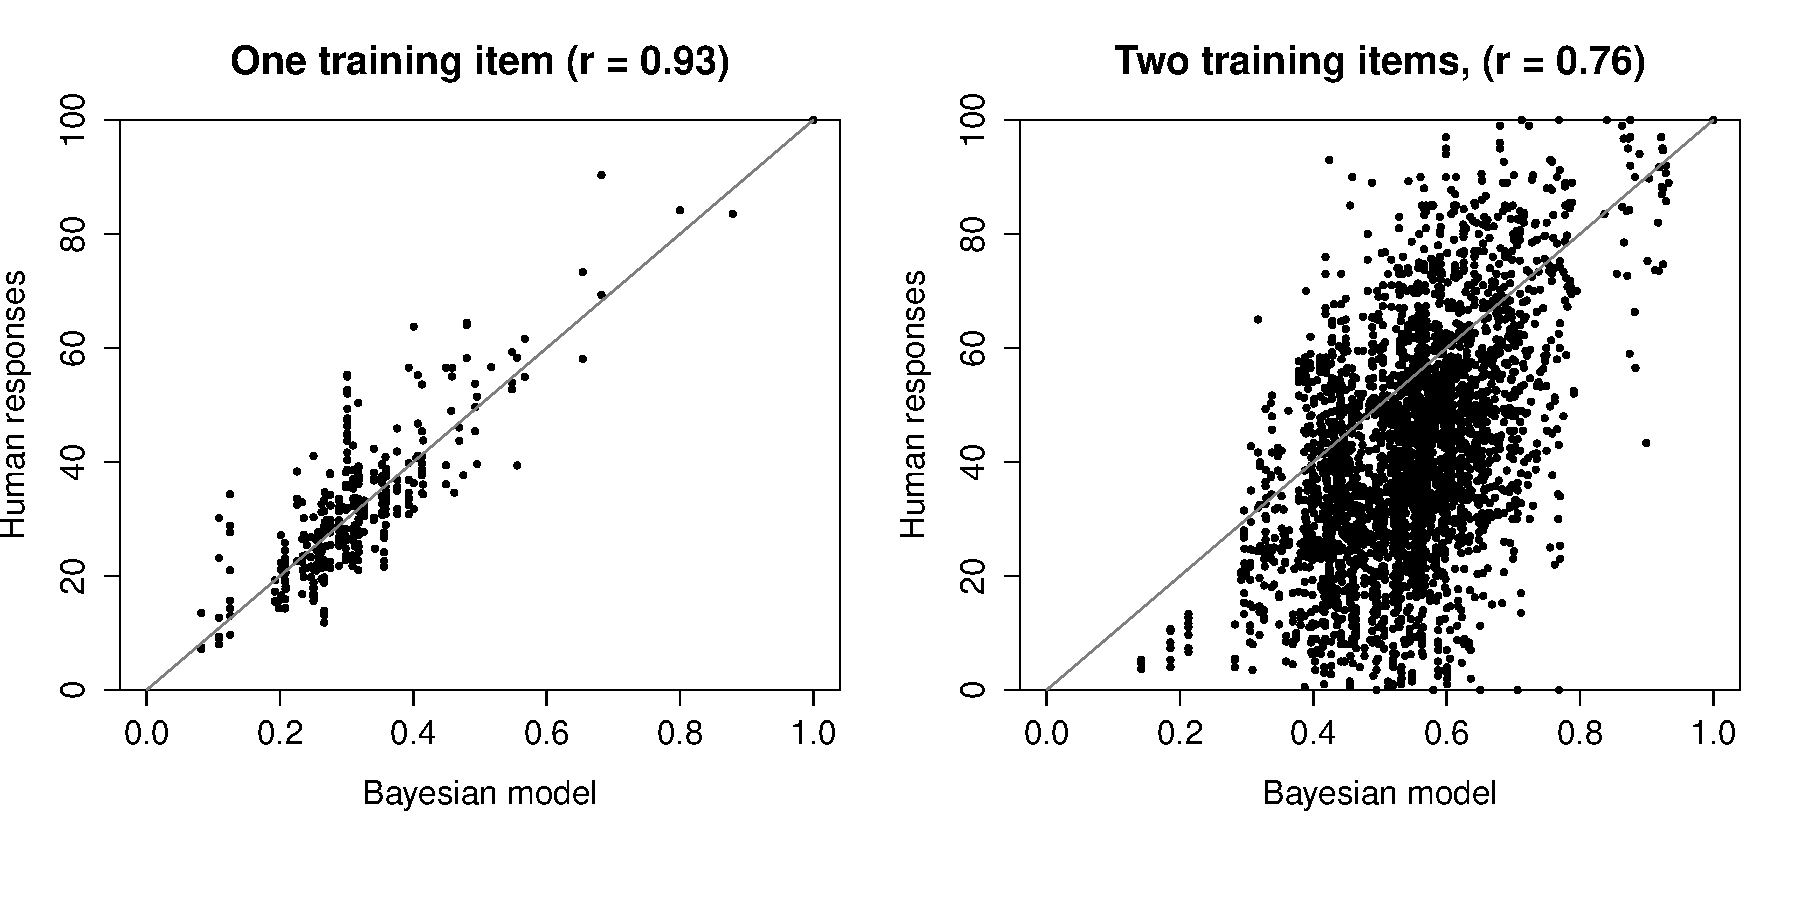
\includegraphics[width=14cm]{generalization_figs/allitems.pdf}
\vspace*{12pt}
\caption{Comparing the model predictions against human responses. The left panel plots all 380 pairs of stimuli for which we obtained generalization judgments, and the right panel plots all 3760 triads for which we did so. The inferred hypothesis space produces generalization probabilities that provide a very good account of those trials in which participants were asked to generalize from a single exemplar (the correlation on the left panel is $r=0.93$), and are adequate ($r=0.76$) when predicting generalizations from multiple items.}
\label{fig:gen_fit}
\end{center}
\end{figure}




%
%\bigskip
%\subsection*{Model predictions}
%Posterior predictive generalization responses from the model are shown in Figure \ref{fig:gen_posterior_pred}. These predictions are based on the mean predicted response across posterior samples of the hypothesis space and prior. The solid line uses posterior samples of $\tau$ to generate noisy predictions using the response model. The dashed line shows the predicted generalizations without response noise. Overall, the model is able to account for the basic pattern in human generalizations across all items. In most cases the model does not appear to capture more subtle effects such as the tightening of generalization gradients. However, it is able to predict broadening of the generalization gradient as shown in the two-item dolphins and wolves subplot.


\subsection*{Discussion}

The central point in our third case study is that using a Bayesian model as a general purpose, descriptive model can be extremely useful as a tool for exploring mental representations. Our application in this instance is a relatively simple example, and is a natural way of extending the framework developed by TG1, but it addresses a fundamental problem in cognitive science, by exploring the hypothesis spaces that underpin human inductive inferences. In light of our results, the utility of Bayesian cognitive models seem obvious. By supplying a probabilistic model for human behavior that links a hypothesis space to an observable response, we can reverse engineer the process and seek to infer the hypothesis space itself. Although we admit to a degree of bias ourselves, it is hard not be interested in results suggesting that people in this task relied more heavily on composite hypotheses and used a weak sampling model. Having found that the Bayesian model works better at capturing generalizations from a single exemplar than from two exemplars, we are motivated to ask why this might be so. We do not know the answer ourselves, but this analysis opened up many useful questions for further exploration.

This case study highlights another point worth making. The descriptive Bayesian approach might provide a partial solution to a common problem within cognitive modeling: the fact that in some situations internal representations, like the hypotheses used by the learner, might not always be recoverable. This occurs when the parameters of the model (which for Bayesian models includes choices of prior and likelihood) are underconstrained by the data \cite<see, e.g.,>{mamassianlandy2010}. The descriptive approach, which performs inference over possible priors and likelihoods, may help by providing researchers with some guidance about whether these choices are reliably constrained by the data.

More importantly for the purposes of the current paper, the importance of these findings seems to be largely unconnected to {\it any} notion of human ``optimality.'' Our analysis used the TG1 model in an entirely pragmatic fashion, as a tool to help us explore people's hypothesis spaces and open up new questions about the inductive biases that guide inductive reasoning. Similarly, it does not seem entirely on point to be asking whether it would be rational for our participants to rely on the categories listed in Table~\ref{table:hypothesis_space}, and thereby make the generalizations they did. To the extent that we have any intuitions about this ourselves, we might be tempted to suggest that people were {\it not} making good judgments: If people really were using a {\it bears} category that lumps \stimulus{koalas} with \stimulus{polar bears} and \stimulus{pandas} as the inductive basis for making generalizations about a biological property (Enzyme-Q), one would hope there is some deeper reason for it other than superficial resemblances. 

However, this is very much besides the point: Our goal with this scenario is to illustrate that the model serves a scientifically useful purpose when used in a purely instrumental fashion. In this application at least, the model does not act as a vehicle for us to justify any claim about the rationality or irrationality of human cognition. It is just a useful tool that allows us to learn about the mind. Indeed, we suggest that Bayesian models are often, in practice, used in exactly this fashion: Probabilistic topic models \cite{steyvers_probabilistic_2007}, structure learning models \cite{kemp_discovery_2008} and models for cross-classification \cite{shafto_probabilistic_2011}, for instance, are all Bayesian frameworks for exploring mental representations that do not seem especially reliant on any notion of ``optimality'' to advance their psychological claims. 
The general philosophy of their approach fits better with the descriptive framework than the Procrustean ``optimal'' framework within which they had to be forced because optimal Bayesian models were the only game in town.

